\chapter[Analýza prestupov a vzdialeností \small{(Marek Šugár)}]{Analýza prestupov a vzdialeností}

Primárnym cieľom tejto kapitoly je detailne analyzovať najkratšie spojenia 
medzi všetkými dostupnými dvojicami letísk (s počtom letísk $3214$ to je dokopy približne 10,33 milióna možných leteckých spojení).
Na problematiku bude nahliadnuté z dvoch hľadísk – priamočiaro cez celkovú vzdialenosť v kilometroch a taktiež cez celkový počet následných
leteckých spojení, resp. počtu nutných prestupov.

V oboch prípadoch k problému pristupujeme výpočtom symetrickej matice najkratších vzdialeností $\mathbf{D}$, kde prvok $\mathbf{D}_{i,j}$ značí minimálnu vzdialenosť
medzi letiskami $i, j$ (v prípade neexistencie cesty, hodnota je $\infty$). Vzhľadom na to je nutné vhodné zvolenie ohodnotenia jednotlivých hrán siete. 

V prestupovej analýze uvažujeme ohodnotenie každej hrany siete rovné $1$ (reprezentácia jedného letu). Výsledná vzdialenostná matica $\mathbf{D} \in \mathbb{R}^{3213 \times 3214}$ 
reprezentuje minimálny počet letov nutných v danom leteckom spojení. Tým pádom možno uvažovať $\mathbf{D} - \mathbf{1}^{3214 \times 3214}$ ako maticu minimálneho počtu prestupov na trasách siete.

V obdobnom zmysle možno uvažovať maticu najkratších vzdialeností. V takom prípade ohodnotenie hrán siete zodpovedá vzdialenosti medzi letiskami v kilometroch. V takom prípade, vzdialenostná matica $\mathbf{D}$
reprezentuje minimálne letecké vzdialenosti na konkrétnej trase.

Na tomto mieste je vhodné poznamenať, že v približne $2.87 \%$ prípadov letecké spojenie neexistuje. Táto časť predstavuje necelých $150$ tisíc trás. 

Pre kompletnosť uvedieme, že výpočet konkrétnych matíc najkratších vzdialeností bola využitá implementácia Dijkstrovho algoritmu, optimalizovaného prioritnou frontou \footnote{Implementácia dostupná v knižnici \texttt{scipy.sparse.csgraph}.}.

\subsection*{Prestupová analýza}
Vizualizácia minimálnej matice prestupov je vyobrazená na Obrázku \ref{fig:layover}. Je možné pozorovať, že drvivá väčšina matice sa vyznačuje relatívne nižším minimálnym potrebným počtom prestupov. Priemerný počet prestupov
je na úrovni $2.997$ – pre akúkoľvek dvojicu letísk je v priemere potrebných aspoň takýto počet prestupov.

Počet letísk, ktoré sú dosiahnuteľné bez prestupu (existuje priama letecká linka) predstavuje približne $0.3573 \%$.

Priemer siete prestupov je $12$ – existuje letecká trasa, ktorá v najkratšom spojení v zmysle prestupov vyžaduje až $12$ prestupov. Jedná sa o spojenie medzi letiskom \textbf{Peawanuck} v Kanade a \textbf{Isiro} v Kongu. Celková vzdialenosť tohto 
leteckého tripu je dovedna $17255.5$ kilometrov.  

\begin{figure}[H]
    \centering
    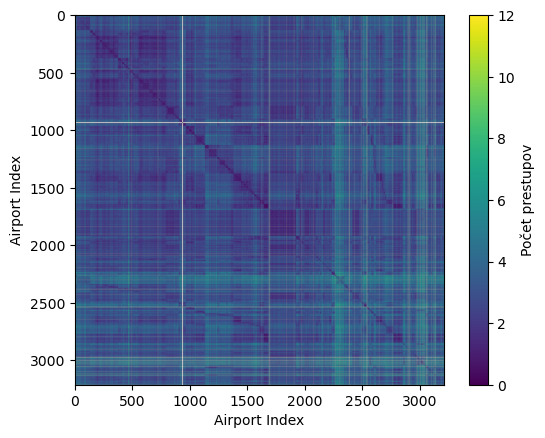
\includegraphics[width=0.6\linewidth]{images/layover.png}
    \caption{\centering Vizualizácia matice minimálneho počtu nutných prestupov.}
    \label{fig:layover}
\end{figure}

V zmysle hlbšej analýzy má zmysel analyzovať aj pravdepodobnostné rozdelenie minimálneho počtu prestupov. Vizualizácia rozdelenia formou histogramu 
je vyobrazená na Obrázku \ref{fig:layover2}. Vo vizualizácii vyobrazujeme aj empirický odhad hustoty rozdelenia dát, konštatujúc, že i napriek tomu, že dáta
vykazujú znaky binomického rozdelenia, nezodpovedali nijakému konvenčnému diskrétnemu rozdeleniu.

\begin{figure}[H]
    \centering
    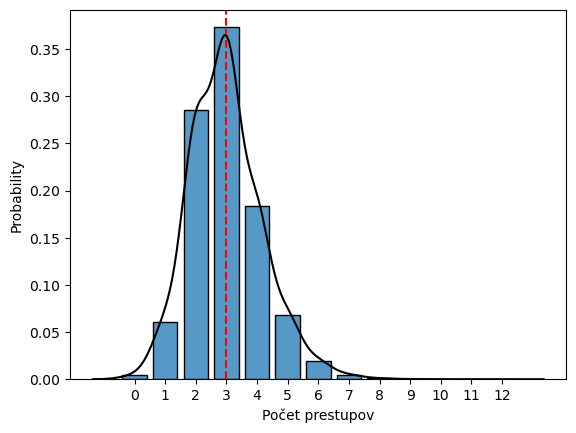
\includegraphics[width=0.55\linewidth]{images/layover_distr.png}
    \caption{\centering Rozdelenie minimálneho nutného počtu prestupov.}
    \label{fig:layover2}
\end{figure}
\newpage
\subsection*{Vzdialenostná analýza}
V rovnakom duchu analýz je možné pristúpiť aj k matici najkratších vzdialeností. Jej samotná vizualizácia sa nachádza na Obrázku \ref{fig:distance}. V tomto prípade je možné pozorovať
už viditeľnejšie koherentné celky, ktoré vykazujú vyššie minimálne vzdialenosti.

\begin{figure}[H]
    \centering
    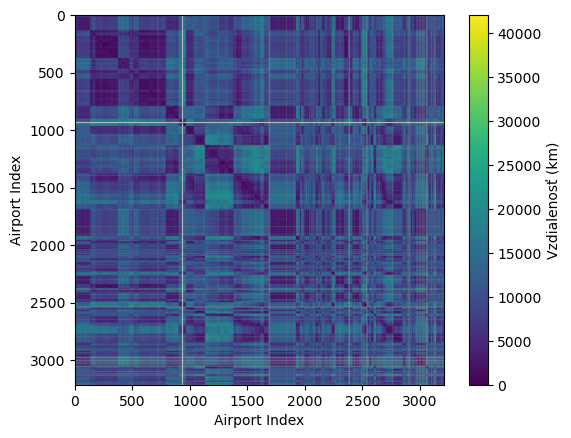
\includegraphics[width=0.7\linewidth]{images/distance.png}
    \caption{\centering Vizualizácia matice minimálnej nutnej vzdialenosti.}
    \label{fig:distance}
\end{figure}

Priemerná vzdialenosť medzi dvojicou letísk je na úrovni zhruba $9946.5$ km. Priemerná vzdialenosť spojení, ktoré sú obslúžiteľné priamym letom 
je $1760.7$ kilometra, čo súčasné dopravné lietadlá dokážu prekonať za približne $2$ hodiny. Najkratšie letecké spojenie je medzi letiskom v britskom meste \textbf{Westray}
a jeho mestskou časťou \textbf{Papa Westray} – dlhé je len $2.8$ km. Naopak najdlhšie priame letecké spojenie má dĺžku $16087.3$ km – medzi leteckou základňou Los Alamitos v Los Angeles a 
letiskom v zambijskej Lusake. 

V zmysle najkratších spojení aj s prestupmi je najdlhšie letecké spojenie medzi tureckým mestom Sinop a mestom Solwesi v Zambii. I napriek tomu, že priame letecké spojenie v tomto prípade 
by malo dĺžku zhruba nad $6000$ km, v zmysle skúmanej logistickej siete je na úrovni až $42076.7$ km. Pre lepšie uchopenie, jedná sa o približne rovníkový obvod Zeme a v prípade (prísne hypotetickom)
by bez prestávky trvala táto trasa moderným diaľkovým lietadlám približne $46$ hodín. Vzhľadom na to, že moderné lietadlá dosahujú dolet najviac približne $15$ tisíc km, jedná sa o veľmi hypotetickú úvahu.
Tento zvlášť neintuitívny výsledok pravdepodobne je spojený so skutočnosťou, že turecké letisko je vojenskou základňou so značne obmedzeným repertoárom letov do iných leteckých základní (opätovne s malým repertoárom spojení), 
čím sa kumulatívne naberala čoraz vyššia celková vzdialenosť, keďže vo viacerých zastávkach letu dochádzalo k dlhým preletom na iné základne.
\newpage
Vizualizácia empirického rozdelenia najkratších vzdialeností medzi letiskami je na Obrázku \ref{fig:distance2}.

\begin{figure}[H]
    \centering
    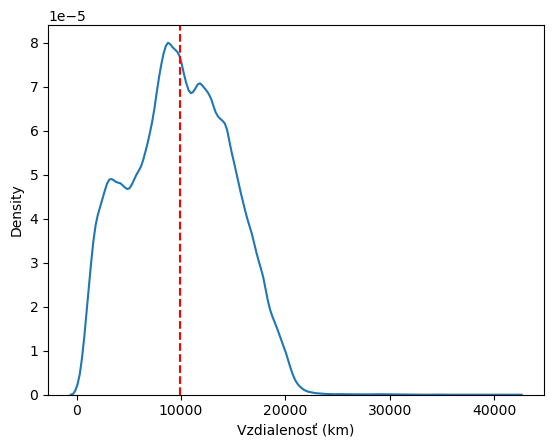
\includegraphics[width=0.7\linewidth]{images/distance_distr.png}
    \caption{\centering Empirické rozdelenie minimálnej nutnej vzdialenosti medzi letiskami.}
    \label{fig:distance2}
\end{figure}

Vzhľadom na relatívne nepravidelný priebeh funkcie empirického rozdelenia, nebolo preukázaná príslušnosť do nijakej konvenčnej rodiny pravdepodobnostného rozdelenia.